\chapterimage{ddd.jpg} % Chapter heading image
\chapter{Întroducere}
\epigraph{Corrige praetertum, praesens rege, cerne futurum - Analizeaza trecutul, conducete de prezent, prevede viitorul }{Lucius Annaeus Seneca minor}
\section{Ce este istoria ?}\index{Ce este istoria ?}
\begin{wrapfigure}[16]{r}{0.2\linewidth} 
    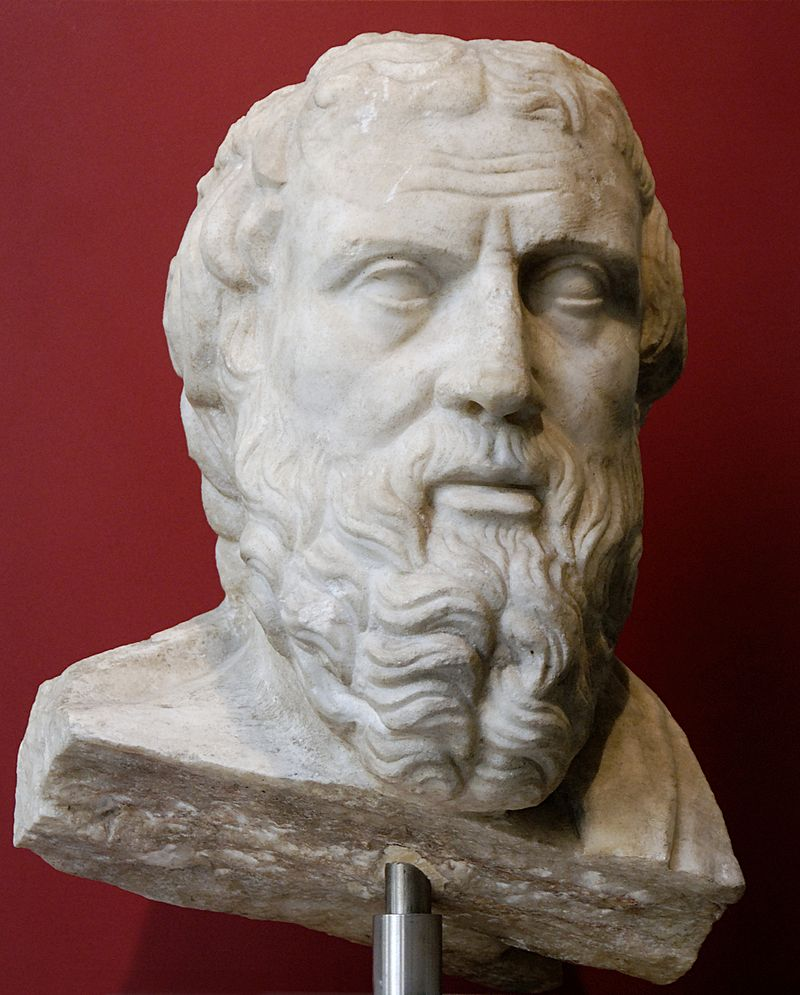
\includegraphics[width=0.27\textwidth]{herodot.jpg}
    \caption{Herodot. Marmură greacă, copie romană a unui original grec de la începutul secolului IV î.Hr.Porta Metronia, Roma.}
    \label{fig:pca}
\end{wrapfigure}
Interesul faţă de trecut este specific rasei umane. Acest interes este greu de explicat doar prin o curiozitate simplă. Faptul că omul însuşi  este o fiinţă istorică.  El se dezvoltă şi să schimbă în timp, fiind produsul a acestei dezvoltări.

Sensul originar al cuvântului "istorie" vine din vechea  greacă  ce insemna "anchetă", "recunoaştere", "înfiinţarea". În antichitate cuvântului "istoria" era folosit ca determinarea cunoştinţelor obţinute prin cercetări în general, adică nu numai despre evenimentele din trecut cum suntem deprinşi să folosim acest cuvînt astăzi. Astfel, Aristotel a folosit acest cuvînt în "Istoria animalelor". De asemenea, îl găsim în imnurile lui Homer, scrierile lui Heraclit şi în textul jurîmântului statului atenian.

Pentru o lungă perioadă de timp istoria nu este văzută ca o ştiinţă, ci  ca un compartiment al literaturii şi artei.Nu întîmplător în mitologia greacă, patronatul asupra istoriei era asigurat de una din muze Clio - o femeie tânără, cu o faţă înspirată, cu un papirus sau pergament în mînă. Numele  muzei Clio - este o derivată  a cuvîntului  grecesc "laudă".

\subsection{Herodot}
Personalitatea lui Herodot, datorită păstrării integrale a operei sale, ni se înfăţişează şi astăzi, aşa cum a fost acum două mii patru sute de ani în urmă, vie, iscoditoare, înclinată să cumpănească oamenii şi faptele lor. Cicero l-a numit pe Herodot "părintele istoriei". Caracterizarea lui Cicero cuprinde o bună parte de adevăr, fără pretenţia să-l identifice pe Herodot cu un adevăreat istoric. Herodot n-a fost altceva decât un cercetător harnic şi talentat, care - depăşind preocupările înguste ale logografilor - a trecut pentru prima oară la compoziţia istorică de proporţii vaste, axată pe un plan bine definit.

Faţă de lucrările predecesorilor săi, Herodot s-a avântat în Istorii la povestirea unui lung şir de evenimente din istoria Orientului şi a Greciei. Nucleul central al acestor evenimente care ţin de secolele al VI-lea şi al V-lea î.e.n., îl constituie războaiele greco-persane şi împrejurările care au dus la izbucnirea ciocnirii între perşi şi daci. Deoarece Herodot a scris cea dintâi istorie cu caracter universal în literatura greacă, afirmaţia lui Cicero apare justificată, caci nimeni până atunci nu se încumetase să închege povestea întâmplărilor din trecu într-o operă de sine stătătoare, străbătută de un fir conducător, şi prea puţini se interesaseră de istoria politică a statelor atunci existente.

\begin{wrapfigure}[11]{l}{0.3\linewidth} 
    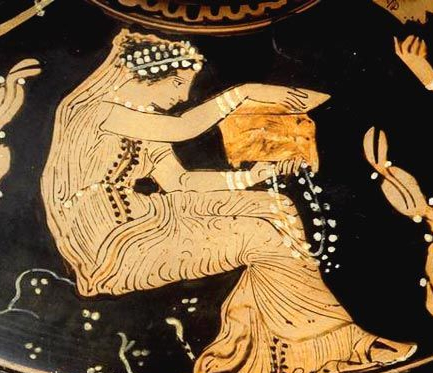
\includegraphics[width=0.27\textwidth]{Clio.jpg}
    \caption{Clio. Fragment de pe un vas grecesc 360 - 340  î.Hr.Porta Musee du Louvre, Paris, Franţa.}
    \label{fig:pca}
\end{wrapfigure}
Datele privitoare la viaţa lui Herodot sunt relativ puţine. Originar din Halicarnas, oraş în Caria colonizat de dorieni, şi integrat ulterior în aria civilizaţiei ioniene, Istoricul a văzut lumina zilei în răstimpul dintre expediţia lui Darius în Grecia (490 î.e.n.) şi ea a lui Xerxes (480 î.e.n.). Deşi n-a fost contemporanul marilor evenimente pe care le-a povestit, amintirea lor - păstrată pretutindeni în lumea elenică în cugetul celor mai vârstnici - i-a folosit cu prisosinţă ca să le descrie cât mai veridic şi plastic.

Din familia sa fruntaşă în Halicarnas, în afară de numele tatălui său, Lyxes, îl cunoaştem pe acela al lui Panyassis, ilustru poet epic, rudă apropiată cu Herodot (poate unchi ). La origine cariană, deşi de mult elenizată, familia lui Herodot se înrudea, în linie paternă, cu casa domnitoare din Halicarnas. Bucurându-se de sprijinul Persiei, casa domnitoare din Halicarnas nu se bucura, în schimb, de simpatia familiilor influente greceşti sau elenizate. Aşa se explică şi vrăjmăşia neîntreruptă arătată de familia lui Herodot tiranilor localnici, din care făcea parte însăşi celebra Artemisia, care l-a ajutat pe Xerxes în bătălia de la Salamina.

Educaţia primită de viitorul istoric al războaielor greco-persane s-a sprijinit pe concepţii de viaţă aristocratice, concepţii preţuite în cercurile influente din Ionia secolelor VI-V î.e.n Herodot a cunoscut îndeaproape creaţia epică şi cea a marilor poeţi lirici, înaintaşii lui, pe care-i şi citează adesea.

Din punct de vedere politic tânărul a participat la lupta dusă de familia sa împotriva tiranului Lygdamis al II-lea, fiul Artemisiei, stăpânitorul Halicarnasului din prima jumătate a secolului al V-lea.

Herodot se stinge din viaţă în jurul anului 425 î.e.n..

Istoriile lui Herodot, deşi în redactarea finală au un plan de concepţie bine definit, nu se înfăţişează ca o unitate desăvârşită. În mai mică măsură decât la epopeile homerice, s-au ivit şi pentru Herodot destule probleme în jurul redactării operei, din care cea mai de seamă rămâne întrebarea dacă autorul şi-a scris dintr-o dată opera, aşa cum o citim noi astăzi, sau a sudat într-un întreg povestiri istorice anterioare.

Subiectul întregii lucrări, care reprezintă, după mărturia autorului, o "cercetare personală", îl găsim enunţat de Herodot chiar la începutul cărţii I: "Herodot din Halicarnas înfăţişează aici rodul cercetărilor sale, pentru ca faptele oamenilor să nu pălească prin trecerea vremii, iar isprăvile mari şi minunate săvârşite şi de greci şi de barbari să nu fie date uitării ; printre altele va pomeni şi pricina pentru care aceştia s-au războit între olaltă".

Când a purces la adunarea materialului pentru vasta sa operă, Herodot a căutat să scrie o istorie cât mai bine documentată în raport cu posibilităţile epocii lui. Pentru aceasta a făcut întinse cercetări personale, a consultat monumente epigrafice şi arhive, s-a informat de la persoanele cele mai competente pe care le-a putut găsi. S.I. Sobolevski face următoarea clasificare pentru izvoarele folosite de Herodot: 1) observaţii personale făcute îndeosebi în cursul călătoriilor, însoţite de cercetări şi concluzii; 2) tradiţia verbală; 3)izvoare scrise.

Cu toată stăruinţa ce a depus-o, el n-a putut totuşi distinge cu fermitate perioada mitologică de cea istorică, nici graniţa dintre legendă şi adevăr. Anumite limite în cercetarea ştiinţifică de care n-a putut trece, limite comune în istoriografia contemporană lui, nu înseamnă că istoricul a fost lipsit de orice discernământ critic. Dimpotrivă, Herodot nu este un credul gata să accepte orice versiune fără să o cântărească, însă informaţia sa intelectuală şi pietatea religioasă l-au îndemnat adesea să accepte ca veridice informaţii care nu pot avea credit sau să tragă concluzii complet eronate.

Herodot obişnuieşte aproape întotdeauna să menţioneze izvorul informativ al faptelor relatate. Informaţia, uriaşă ca volum, pe care se sprijină compoziţia Istoriilor, se împarte în două categorii distincte: directă - fapte şi lucruri cunoscute sau văzute de istoric personal, indirectă - fapte şi lucruri aflate de la alţii. Concluzii deduse de Herodot însuşi pe calea raţionamentelor sunt comune ambelor categorii de informaţie; în majoritatea lor însă, ele nu pot sta în picioare, cum e cazul în cartea I, cap. CXCVI, de pildă, sau în cartea a II-a, cap. XXIV.

În istoria universală pe care a scirs-o Herodot, în munca uriaşă de unificare a părţilor ei componente nu putea lipsi o anumită concepţie asupra desfăşurării procesului istoric; diversitatea stadiilor orânduirii primitive şi sclavagiste pe care istoricul le-a luat în consideraţie l-au silit, la rândul lor, să reflecteze asupra dezvoltării societăţii omeneşti.\footnote{Herodot - Istorii, Ed. Ştiinţifică, 1961} 
\newpage

\section{Istoria ca ştiinţă}\index{Istoria ca ştiinţă}
\epigraph{Historia est Magistra Vitae}{Marcus Tullius Cicero}
After I arrived and had my first meeting with Pauline, she explained me a general idea of what she wanted and shared me some more papers (about multi-wavelenght studies), I read the information and came up with the objective.

\begin{itemize}
\item Find out a method to transform data from a high dimensional dataset (FITS cube or any other data arrangement) to a low dimensional understandable information (graphs, clusters).
\end{itemize}

This means that from multiple images with different wavelengths of the same target apply an algorithm to find the hidden patterns that lie hidden between them.

\section{Ştiinţele istorice}\index{Ştiinţele istorice}
Ok, here is where I explain from where this is going to start, at that time I just had a microcontrollers and engineering design course my mind was set completelly to find appplicable theories and create uselful things with them, which is the complete opposite of how astronomy works. First, there's no way to test an experiment with galaxies and most of the information is fuzzy and subjective (not all). The process of having an, let's say \emph{astronomy idea} is a result of applying all your physics knowledge and consider the \textbf{cosmological principle},
\begin{quote}
The (testable) assumption that the same physical laws that apply here and now also apply everywhere and at all times, and that there are no special locations or directions in the universe.
\end{quote}

That's how science is made, thinking and testing and thinking again, creating your own scientific method, comming up with hypothesis, learning what might work and what not, using your insticts. 

Well, before comming here I didn't think like that, it was just all about being super productive and thinking about doing robots and all kinds of devices with sensors. I had some experience programming in C/C++, no computer science backgound and I had never had an astronomy course.

This report was written in order to help someone to continue researching about data mining techniques applied in Astronomy, I explain how did I come up with the clustering techniques, my hypothesis, some tests and other ideas I have had, I hope this can help anyone and the research is continued. Anything you may need/questions do not hesitate to contact me, my e-mail address is: \emph{mrs.petzl@gmail.com}, also s part of my own documentation I created a GitHub page where you can download all the codes I programmed and find more information. The link to this page is: \url{https://github.com/LaurethTeX/Clustering}, from the \textsc{readme} file you can acces to all the pages, take your time to surf.
%------------------------------------------------

\subsection{References}\index{References}

Since I found so much good information about pretty much everything I wanted to know about, I will just create a remark and let you know where you can find more specific information about, just like below.


\begin{expli}
For more information about the cosmological principle, review Chapter 1: Why Learn Astronomy?, page 10, from \textbf{21st Century Astronomy}, \textit{Hester | Smith | Blumenthal | Kay | Voss}, Third Edition, 2010.
\end{expli}


%This statement requires citation \cite{book_key}; this one is more specific \cite[122]{article_key}.
